\documentclass[14p, hyperref={unicode}]{beamer}

\usepackage[T1]{fontenc}
\usepackage[utf8]{inputenc}
\usepackage[slovene]{babel}
\usepackage{lmodern}
\usepackage{array}
\usepackage{epsdice}
\usepackage{makecell}
\usepackage{bm}
\usepackage{xcolor}
\usepackage{amsmath}
\usepackage{amsfonts}
\usepackage{amssymb}
% \usepackage{enumitem}
\usepackage{pifont}



\setbeamerfont{caption}{size=\scriptsize}



\newcolumntype{P}[1]{>{\centering\arraybackslash}p{#1}}


\usetheme{Berlin}
\definecolor{UBCblue}{rgb}{0.04706, 0.13725, 0.26667}
\usecolortheme[named=UBCblue]{structure}

\useinnertheme[shadows]{rounded}
\useoutertheme{infolines}

\usepackage{palatino}
\usefonttheme{serif}

\setbeamertemplate{enumerate item}{(\alph{enumi})}
\beamertemplatenavigationsymbolsempty

\graphicspath{{beamer/}}

\renewcommand{\raggedright}{\leftskip=0pt \rightskip=0pt plus 0cm}

\title[Model napovedi odjema]{MODEL NAPOVEDI ODJEMA ELEKTRIČNE ENERGIJE}
\subtitle{Matematika z računalnikom 2023/24}
\author[Karolina Šavli]{Karolina Šavli \\ Mentorstvo: dr. Blaž Krese in Rok Geršak iz GEN-I}
\date{6.~junij 2024}


\begin{document}


% \begin{figure}
%     \centering
%     \includegraphics[width=0.85\textwidth]{razvrstitev_v_skupine.png}
% \end{figure}




% ===================================================================


\begin{frame}

    \titlepage

\end{frame}


% -------------------------------------------------------------------


\begin{frame}

    \frametitle{Kratek pregled predstavitve}
    \tableofcontents

\end{frame} 


% ===================================================================

 
\section{Podatki in cilj projektne naloge}


% -------------------------------------------------------------------


\begin{frame}

    \frametitle{Predstavitev podatkov}

    \uncover<1->{

    \begin{itemize}
        \item Podjetje \href{https://gen-i.si/}{GEN-I} je pripravilo tabelo podatkov:

    \begin{figure}
        \centering
        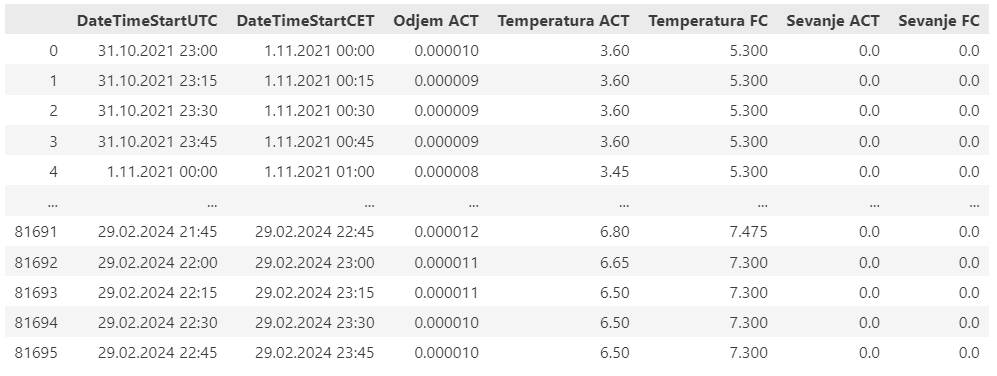
\includegraphics[width=0.9\textwidth]{tabela.png}
    \end{figure}

    \item Obdobje od $1.~\text{novembra}~2021$ do $29.~\text{februarja}~2024$,
    na $15$ minut

    \item Stolpec \texttt{Odjem ACT} sem pomnožila s $10^6$
    
    }
    
    \uncover<2->{

    \item \textbf{Cilj projekta}: sestaviti model, ki bo kar se da točno 
    napovedal odjem električne energije \textbf{gospodinjskih odjemalcev} za naslednji dan

    }

    \end{itemize}
    
\end{frame}


% ===================================================================


\section{Osnovna analiza podatkov}


% -------------------------------------------------------------------


\subsection{Odjem električne energije}

\begin{frame}
    
    \frametitle{Odjem električne energije} 

    \begin{figure}[h!]
        \centering
        \caption{Odjem električne energije, 2021-2024}\par\medskip
        \label{fig:odjem_EE}
        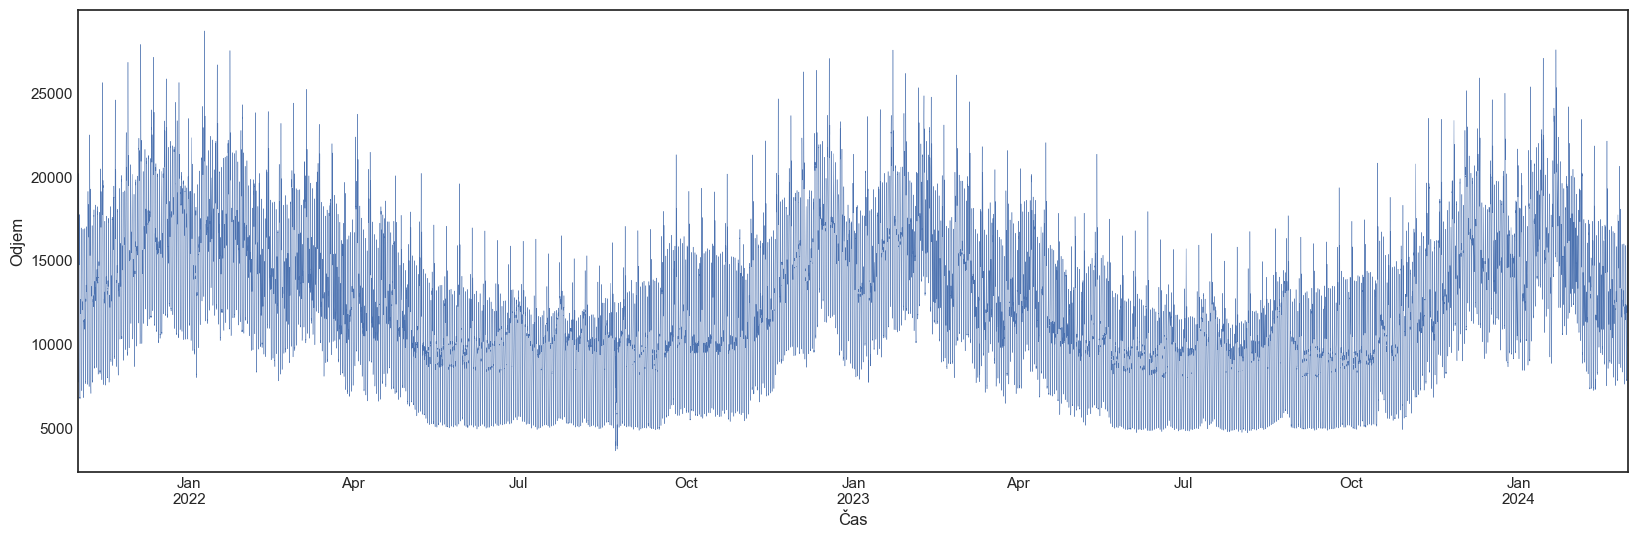
\includegraphics[width=0.9\textwidth]{odjem_EE.png}
    \end{figure}

    \begin{itemize}
        \item Odjem je znatno večji jeseni in pozimi
    \end{itemize}

    \vfill

\end{frame}


% -------------------------------------------------------------------


\begin{frame}
    
    \frametitle{Odjem električne energije \textbf{na ravni tedna}} 

    \begin{figure}[h!]
        \centering
        \caption{Odjem električne energije po urah, drugi teden septembra 2023}\par\medskip
        \label{fig:odjem_teden}
        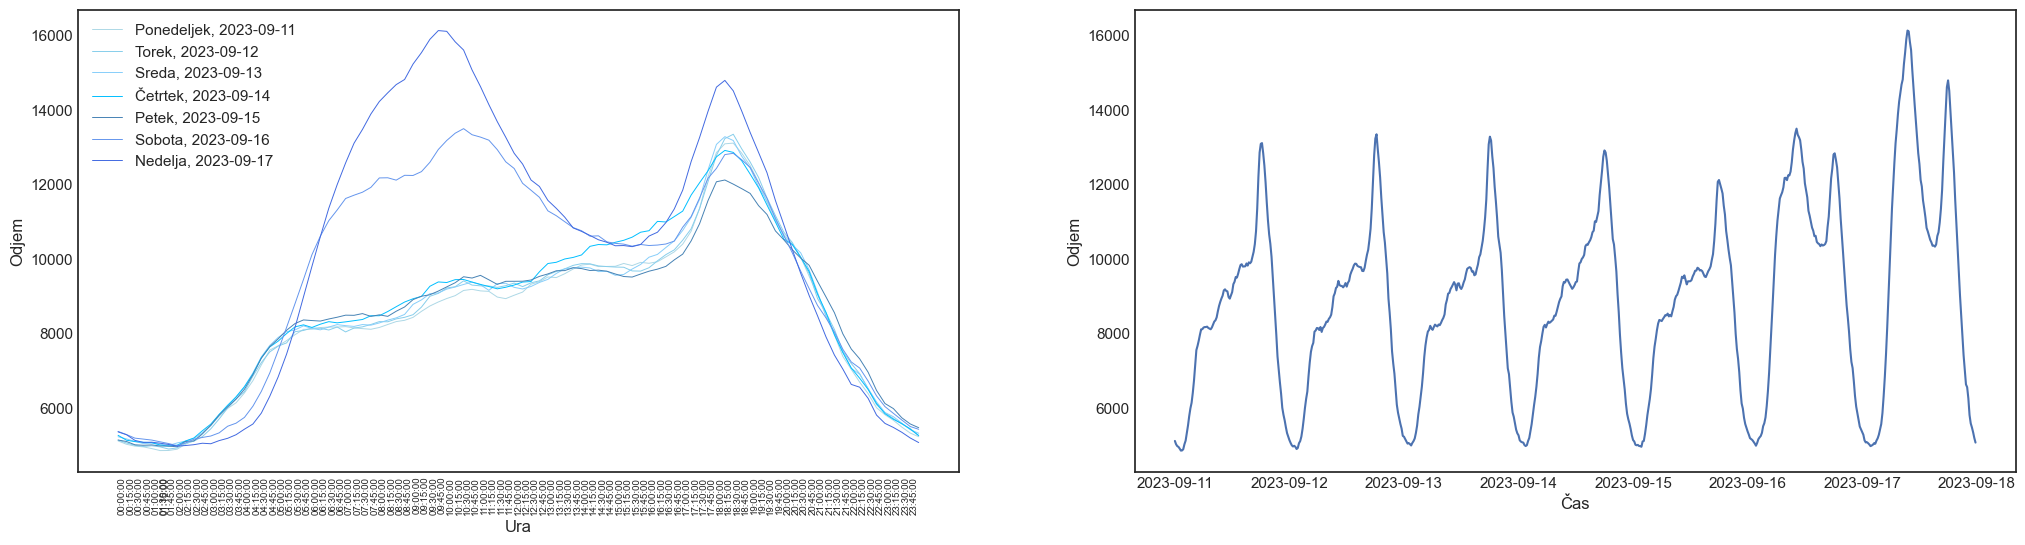
\includegraphics[width=0.9\textwidth]{odjem_teden.png}
    \end{figure}

    \begin{itemize}
        \item Med tednom: en višek
        \item Vikend: dva viška
        \item Sezonskost na dnevni ravni
    \end{itemize}

    \vfill

\end{frame}


% -------------------------------------------------------------------


\subsection{Povezava med odjemom in temperaturo ter sevanjem}

\begin{frame}
    
    \frametitle{Povezava med odjemom in temperaturo ter sevanjem} 

    \uncover<1->{

    \begin{figure}[h!]
        \centering
        \caption{Povezava med odjemom in temperaturo ter sevanjem, 2021-2024}\par\medskip
        \label{fig:temp_sevanje}
        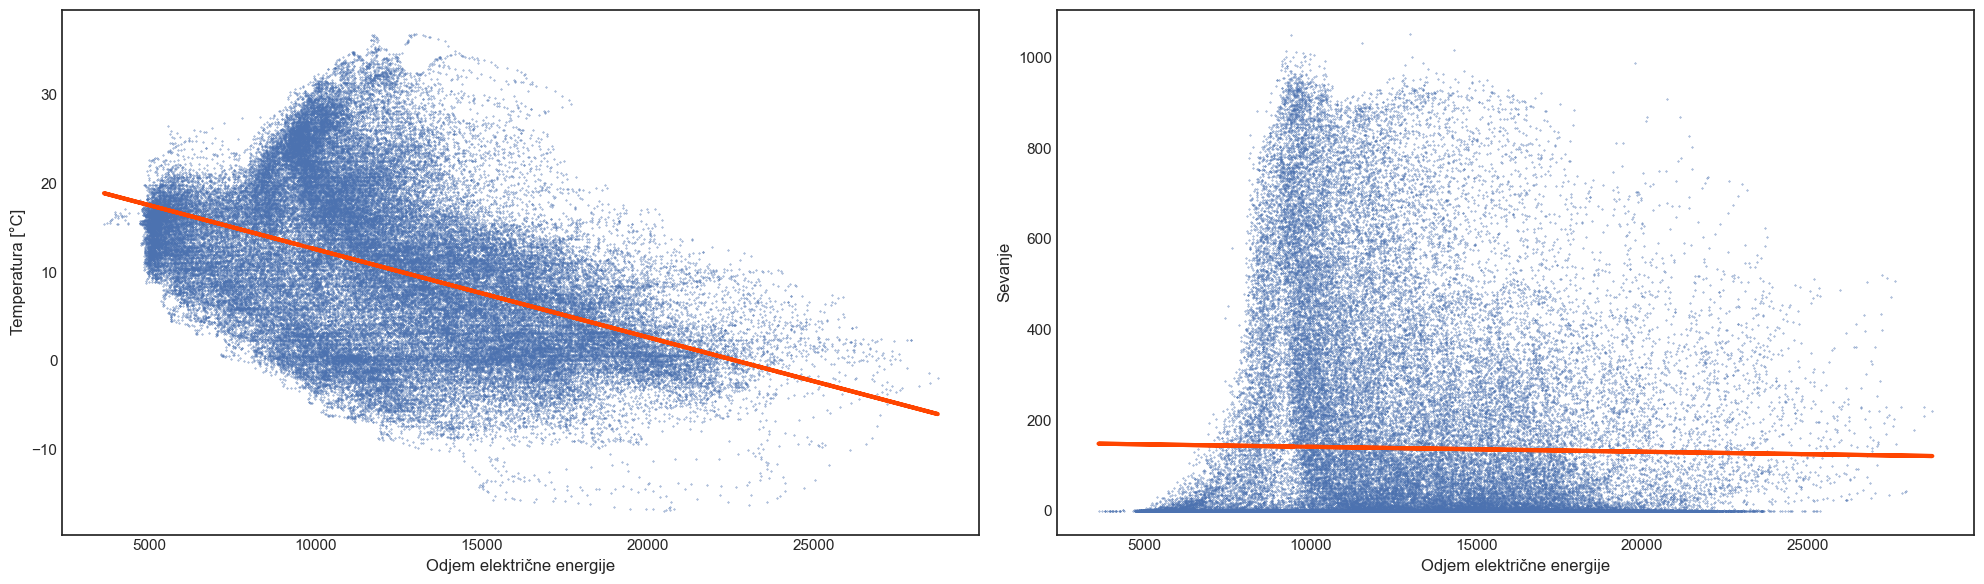
\includegraphics[width=0.9\textwidth]{temp_sevanje.png}
    \end{figure}

    \begin{itemize}
        \item $\uparrow$ temperatura $\rightarrow$ odjem $\downarrow$
        \item Povezava s sevanjem ni razvidna
        
    }

    \uncover<2->{

        \item Temperaturo in sevanje bomo v model vključili kot eksogeni spremenljivki
    
    }

    \end{itemize}

    \vfill

\end{frame}


% ===================================================================


\section{Napredna analiza podatkov}


% -------------------------------------------------------------------


\subsection{Izbira družine modelov}

\begin{frame}
    
    \frametitle{Izbira družine modelov} 

    \uncover<1->{

    \begin{itemize}
        \item Gre za časovno vrsto $\rightarrow$ uporaba teorije časovnih vrst }
        \uncover<2->{
        \item Časovna vrsta odjema: visofrekvenčna, ima sezonsko komponento in njeno povprečje ni konstantno 
        \item Družina modelov ARMA }
    \end{itemize}

\end{frame}


% -------------------------------------------------------------------


\begin{frame}
    
    \frametitle{Družina modelov ARMA} 

    \uncover<1->{ 

    \begin{itemize}
        \item Model ARMA }
        \uncover<2->{
        \item Nimamo popolnoma stacionarnih podatkov $\rightarrow$ ARIMA
    \end{itemize}

    \small
    \begin{equation*}
        X_t = \mu + \sum_{i=1}^{p}{\varphi_i X_{t-i}} + \sum_{i=1}^{q}{\theta_i \varepsilon_{t-i}} +  \varepsilon_t\,
    \end{equation*}
    \normalsize

        }

    \uncover<3->{ 

    \begin{itemize}
        \item Imamo sezonsko komponentno $\rightarrow$ {\color{blue} SARIMA}
    \end{itemize}

    \small
    \begin{equation*}
        X_t = \mu + \sum_{i=1}^{p}{\varphi_i X_{t-i}} + \sum_{i=1}^{q}{\theta_i \varepsilon_{t-i}} + \color{blue} \sum_{i=1}^{P}{\phi_i X_{t-S}} + \sum_{i=1}^{Q}{\Theta_i \varepsilon_{t-S}}  \color{black} +  \varepsilon_t\,
    \end{equation*}
    \normalsize

    } 

    \uncover<4->{

    \begin{itemize}
        \item Vključitev eksogenih podatkov $\rightarrow$ {\color{red} SARIMAX}
    \end{itemize}
    
    \small
    \begin{equation*}
        X_t = \mu + \sum_{i=1}^{p}{\varphi_i X_{t-i}} + \sum_{i=1}^{q}{\theta_i \varepsilon_{t-i}} + \color{blue} \sum_{i=1}^{P}{\phi_i X_{t-S}} + \sum_{i=1}^{Q}{\Theta_i \varepsilon_{t-S}}  \color{red}  + \sum_{r=1}^{R}{\beta_i Y_{i_{t}}} \color{black} +  \varepsilon_t\,
    \end{equation*}
    \normalsize

    }

\end{frame}


% -------------------------------------------------------------------


\begin{frame}
    
    \frametitle{Model SARIMAX-GARCH} 

    \uncover<1->{

    \begin{itemize}
        \item Družina modelov ARMA ima težavo predvsem pri napovedih časovnih vrst, ki se jim  
        skozi čas spreminja varianca $\rightarrow$ povezava z modelom {\color{green} GARCH} }
        \uncover<2->{
        \item Dobimo model SARIMAX(p,d,q)(P,D,Q)[S]-GARCH($p_G$,$q_G$):
    \end{itemize}

    \small
    \begin{equation*}
        X_t = \mu + \sum_{i=1}^{p}{\varphi_i X_{t-i}} + \sum_{i=1}^{q}{\theta_i \varepsilon_{t-i}} + \color{blue} \sum_{i=1}^{P}{\phi_i X_{t-S}} + \sum_{i=1}^{Q}{\Theta_i \varepsilon_{t-S}}  \color{red}  + \sum_{r=1}^{R}{\beta_i Y_{i_{t}}} \color{green} + \sqrt{\sigma_t} z_t \color{black} \,,
    \end{equation*}
    \normalsize

    kjer je $\color{green} \sigma^2_t = \omega + \sum_{i=1}^{p_G}{\alpha_i \varepsilon_{t-i}^2} + \sum_{i=1}^{q_G}{\beta_i \sigma_{t-i}^2} \,$, 
    $\color{green} \sigma^2_t$ je pogojna varianca ob času $\color{green} t$, $\color{green} \varepsilon_t$ pa 
    beli šum ob času $\color{green} t$ in $\color{green} \color{green} z_t \sim \text{NEP}(0,1)$. }

\end{frame}


% -------------------------------------------------------------------


\subsection{Odstranitev sezonskosti in pridobitev stacionarnosti}

\begin{frame}
    
    \frametitle{Originalna časovna vrsta} 

    \begin{itemize}
        \item $W_t$ \dots~ originalna časovna vrsta odjema električne energije
    \end{itemize}

    \begin{figure}[h!]
        \centering
        \caption{Odjem električne energije, 2021-2024}\par\medskip
        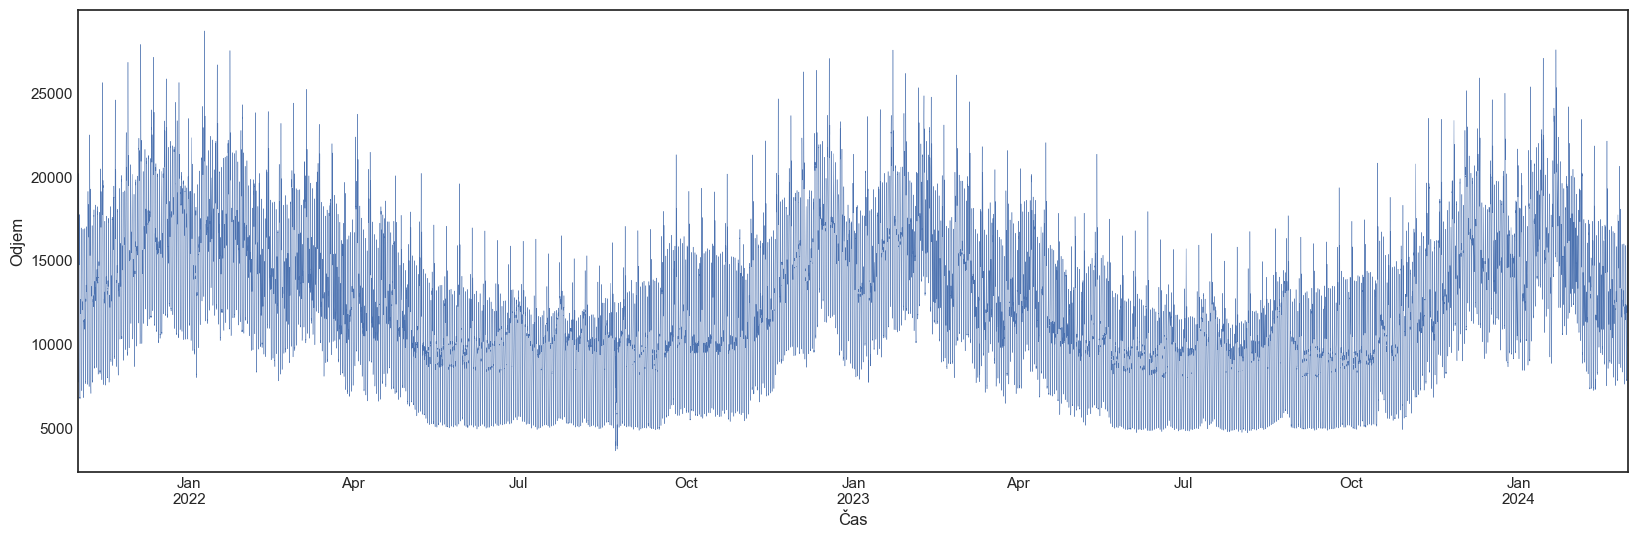
\includegraphics[width=0.9\textwidth]{odjem_EE.png}
    \end{figure}

    \begin{itemize}
        \item Podatki so volatilni $\rightarrow$ naredimo \textbf{logaritmične donose} 
        (ang. \emph{log returns}): $ Y_t = \ln \left( \frac{W_t}{W_{t-1}} \right) $
    \end{itemize}



\end{frame}


% -------------------------------------------------------------------


\begin{frame}
    
    \frametitle{Log returns} 

    \begin{figure}[h!]
        \centering
        \caption{Logaritmični donosi odjema električne energije, 2021-2024}\par\medskip
        \label{fig:log_returns}
        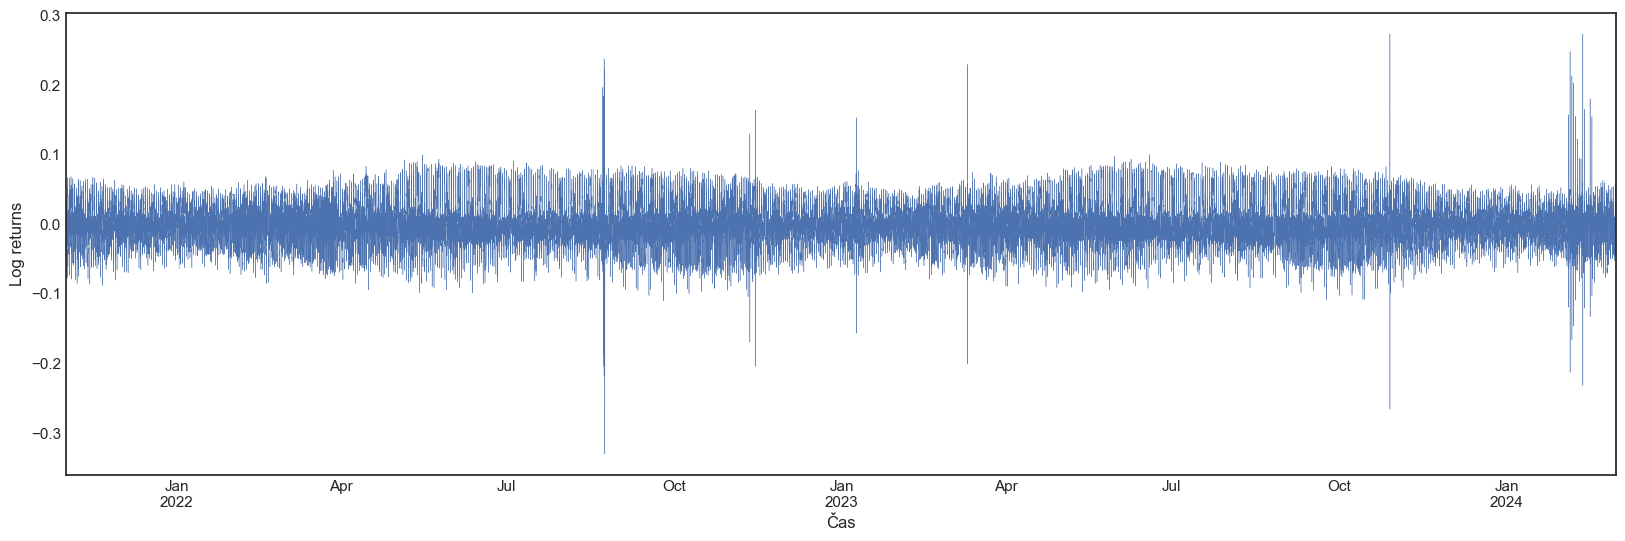
\includegraphics[width=0.9\textwidth]{log_returns.png}
    \end{figure}

\end{frame}


% -------------------------------------------------------------------


\begin{frame}
    
    \frametitle{ACF in PACF za Log returns} 

    \begin{figure}[h!]
        \centering
        \caption{Vzorčna avtokorelacijska in parcialna avtokorelacija funkcija logaritmičnih donosov}\par\medskip
        \label{fig:log_returns_acf_pacf}
        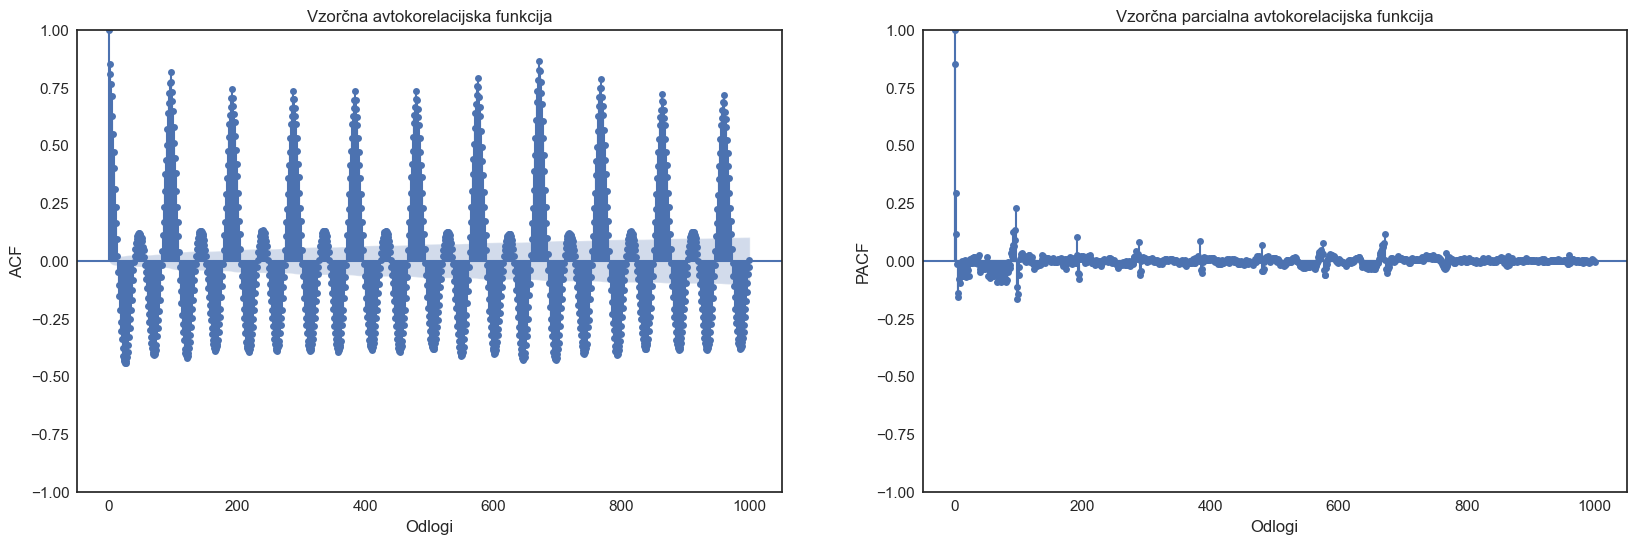
\includegraphics[width=0.9\textwidth]{log_returns_acf_pacf.png}
    \end{figure}

    \begin{itemize}
        \item Časovna vrsta \textbf{ni} stacionarna
        \item Sezonska komponentna: 96 (ravno en dan) $\rightarrow$ sezonsko diferenciramo
    \end{itemize}
    
\end{frame}


% -------------------------------------------------------------------


\begin{frame}
    
    \frametitle{Sezonska diferenciacija} 

    \begin{itemize}
        \item Podatke \textbf{sezonsko diferenciramo}
        \item Nova časovna vrsta: $Z_t = Y_t - Y_{t-96} = \bigtriangledown_{96}Y_t$.
    \end{itemize}

    \begin{figure}[h!]
        \centering
        \caption{Časovna vrsta $Z_t$, 2021-2024}\par\medskip
        \label{fig:ts_diff}
        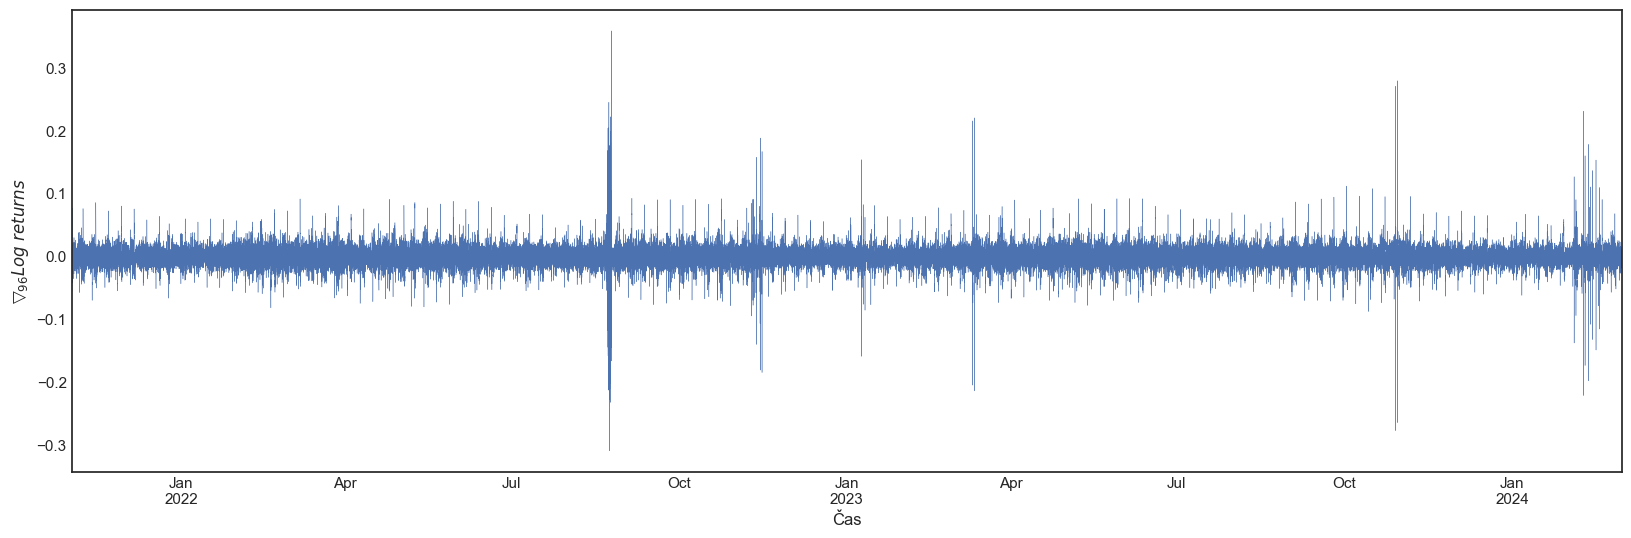
\includegraphics[width=0.9\textwidth]{ts_diff.png}
    \end{figure}

\end{frame}


% -------------------------------------------------------------------


\begin{frame}
    
    \frametitle{ACF in PACF časovne vrste $Z_t$} 

    \begin{figure}[h!]
        \centering
        \caption{Vzorčna avtokorelacijska in parcialna avtokorelacija funkcija časovne vrste $Z_t$}\par\medskip
        \label{fig:ts_diff_acf_pacf}
        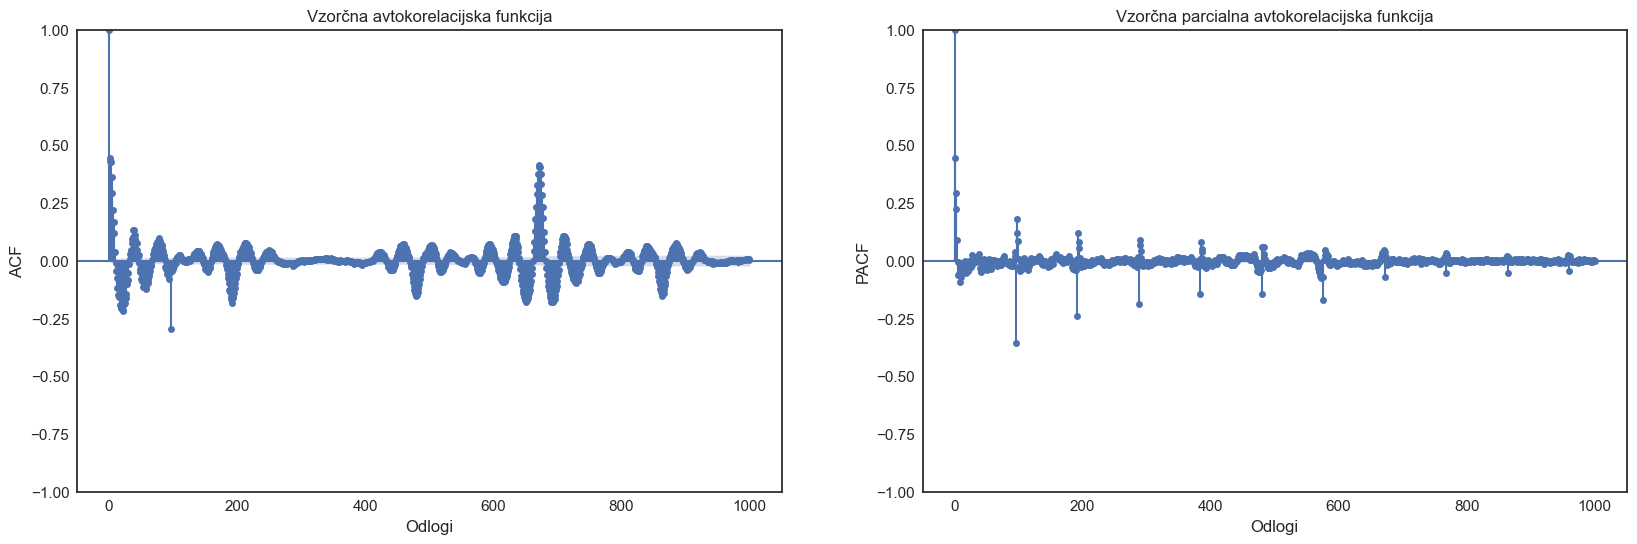
\includegraphics[width=0.9\textwidth]{ts_diff_acf_pacf.png}
    \end{figure}

    \begin{itemize}
        \item Ponavljanje vzorca $\rightarrow$ vrsta še kar ni stacionarna $\rightarrow$ \emph{navadno} diferenciramo
    \end{itemize}
    
\end{frame}


% -------------------------------------------------------------------


\begin{frame}
    
    \frametitle{\emph{Navadna} diferenciacija} 

    \begin{itemize}
        \item Dobimo časovno vrsto $X_t = Z_t - Z_{t-1} = \bigtriangledown{Z_t}$
    \end{itemize}

    \begin{figure}[h!]
        \centering
        \caption{Časovna vrsta $X_t$, 2021-2024}\par\medskip
        \label{fig:ts_diff_2}
        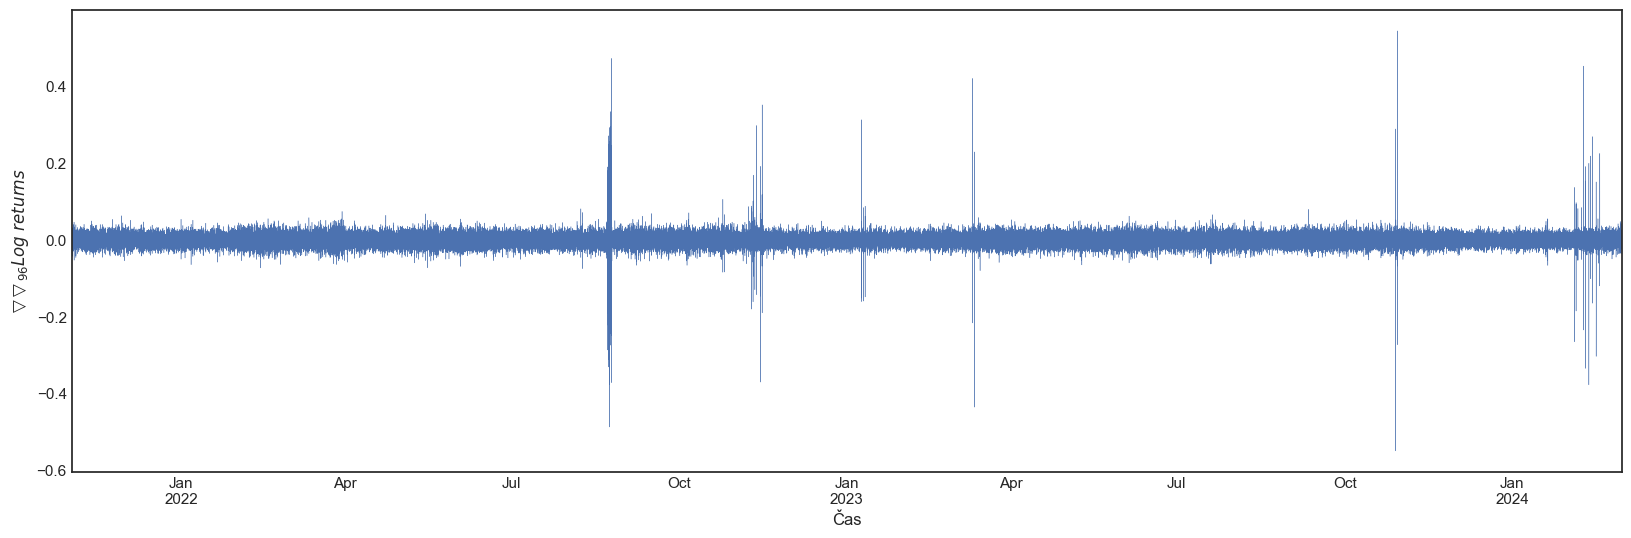
\includegraphics[width=0.9\textwidth]{ts_diff_2.png}
    \end{figure}
    
\end{frame}


% -------------------------------------------------------------------


\begin{frame}
    
    \frametitle{ACF in PACF časovne vrste $X_t$} 

    \begin{figure}[h!]
        \centering
        \caption{Vzorčna avtokorelacijska in parcialna avtokorelacija funkcija časovne vrste $X_t$}\par\medskip
        \label{fig:ts_diff_2_acf_pacf}
        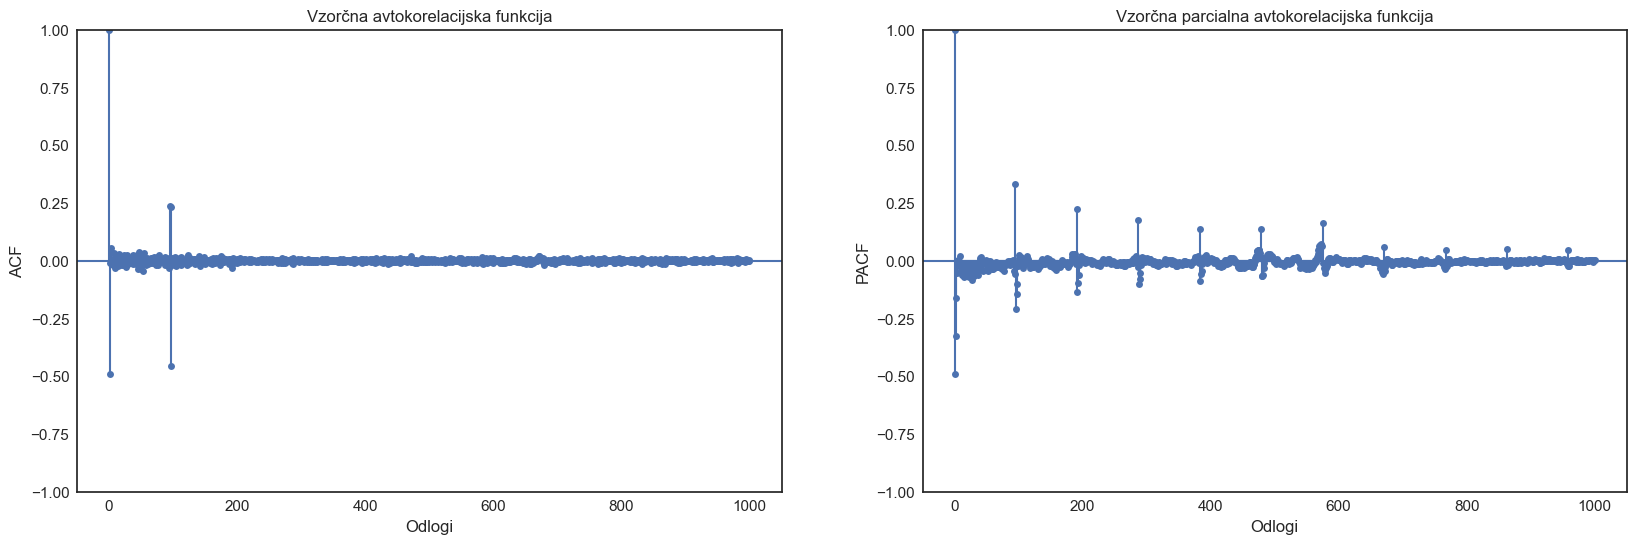
\includegraphics[width=0.9\textwidth]{ts_diff_2_acf_pacf.png}
    \end{figure}

    \begin{itemize}
        \item Časovna vrsta je stacionarna
    \end{itemize}
    


\end{frame}


% -------------------------------------------------------------------


\begin{frame}
    
    \frametitle{} 

    \uncover<1->{

    \textbf{Kaj smo torej naredili z originalno časovno vrsto?}

    Originalna časovna vrsta $\rightarrow$ Log returns $\rightarrow$ sezonsko diferencirali
    $\rightarrow$ \emph{Navadno} diferencirali

    }

    \uncover<2->{

    \vfill
    
    \textbf{Naslednji korak:}

    S pomočjo ACF in PACF stacionarne časovne vrste $X_t$ določimo parametre modela SARIMAX 

    }

\end{frame}


% -------------------------------------------------------------------


\subsection{Identifikacija modela SARIMAX}

\begin{frame}
    
    \frametitle{Določitev parametrov modela SARIMAX} 

    \uncover<1->{

    \Large
    \textbf{SARIMAX{\color{orange}(p,d,q)}{\color{purple}(P,D,Q)[S]}}
    \normalsize

    \vfill

    \begin{itemize}
        \item Enkrat smo sezonsko diferencirali $\rightarrow$ $\color{purple} \text{D} = 1$
        \item Enkrat smo navadno diferencirali $\rightarrow$ $\color{orange} \text{d} = 1$
        \item Perioda je $96$ $\rightarrow$ $\color{purple} \text{S} = 96$
    \end{itemize}

    }

    \uncover<2->{

    \vfill

    Za določitev {\color{purple}sezonskih} parametrov {\color{purple}P} in {\color{purple}Q} gledamo korelacije pri odlogih, ki so večkratniki periode S

    }

\end{frame}


% -------------------------------------------------------------------


\begin{frame}
    
    \frametitle{} 

    \Large
    \textbf{SARIMAX{\color{orange}(p,1,q)}{\color{purple}(P,1,Q)[96]}}
    \normalsize

    \begin{figure}[h!]
        \centering
        \caption{Vzorčna avtokorelacijska in parcialna avtokorelacija funkcija časovne vrste $X_t$}\par\medskip
        \label{fig:ts_diff_2_acf_pacf}
        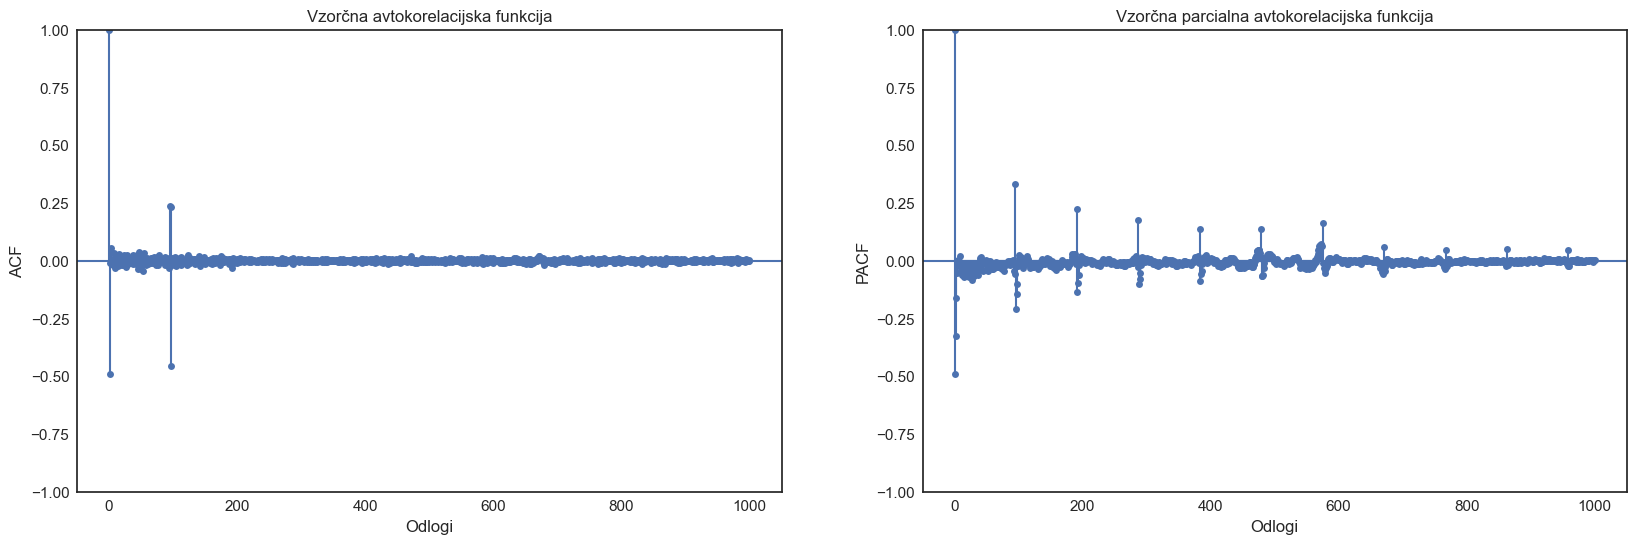
\includegraphics[width=0.9\textwidth]{ts_diff_2_acf_pacf.png}
    \end{figure}

    \begin{itemize}
        \item PACF $\rightarrow$ {\color{purple} P je vsaj 1}
        \item ACF $\rightarrow$ $\color{purple} \text{Q} = 1$
    \end{itemize}

\end{frame}


% -------------------------------------------------------------------


\begin{frame}
    
    \frametitle{} 

    \Large
    \textbf{SARIMAX{\color{orange}(p,1,q)}{\color{purple}(P,1,1)[96]}}
    \normalsize

    \begin{figure}[h!]
        \caption{Vzorčna avtokorelacijska in parcialna avtokorelacija funkcija vrste $X_t$, odlogi do 100}\par\medskip
        \centering
        \label{fig:ts_diff_2_acf_pacf_do_100}
        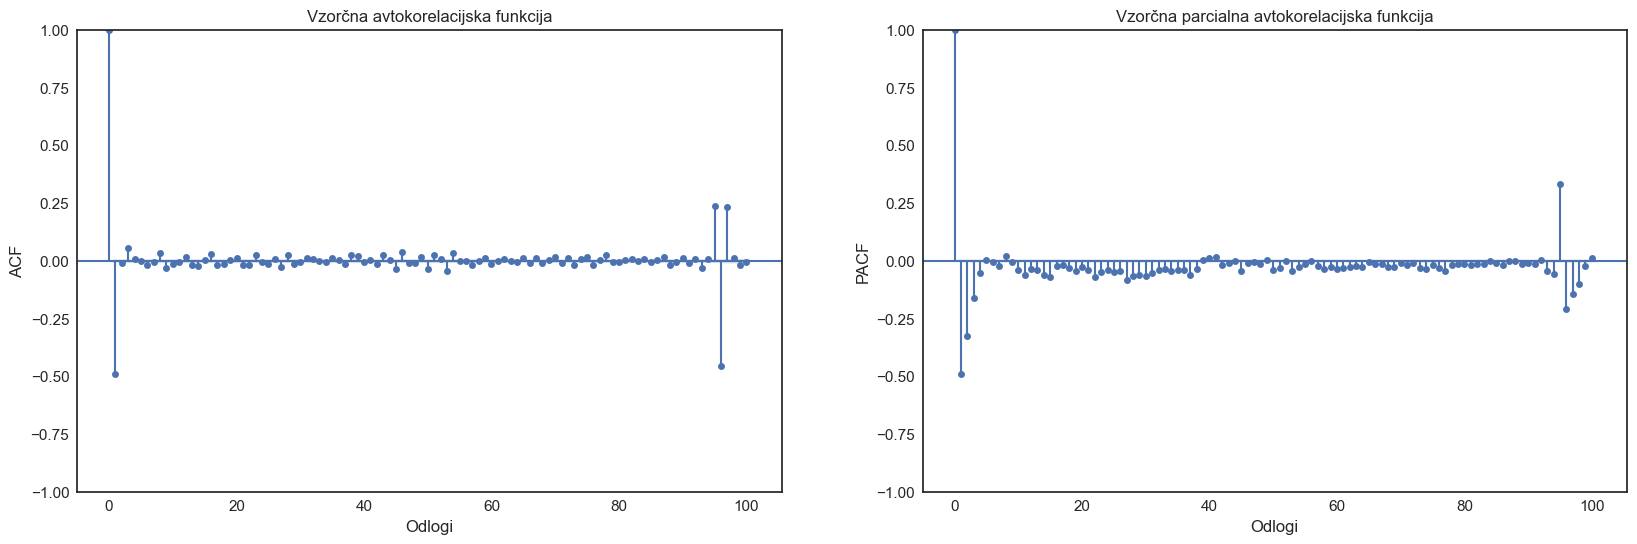
\includegraphics[width=0.9\textwidth]{ts_diff_2_acf_pacf_do_100.png}
    \end{figure}

    Za določitev {\color{orange}nesezonskih} parametrov {\color{orange}p} in {\color{orange}q} gledamo ACF in PACF do prve periode (torej do odloga 96)

    Večja korelacija pri prvih nekaj urah in v uri tik pred periodo $\rightarrow$
    {\color{orange}vključimo prvih nekaj 15-minutnih intervalov}

\end{frame}


% -------------------------------------------------------------------


\begin{frame}
    
    \frametitle{Izbira modela SARIMAX na podlagi vrednosti kriterija AIC} 

    \uncover<1->{

    \begin{itemize}
        \item Eksogeni spremenljivki: temperatura in sevanje
        \item Model sem trenirala na $75~\%$ podatkih }
        \uncover<2->{
        \item Vrednosti kriterije AIC za izbrane modele:
    \end{itemize}

    
\begin{table}[!ht]
    \centering
    \footnotesize
    \begin{tabular}{c|c}
        Model & AIC \\ \hline
        SARIMAX(1,1,0)(0,1,0)[96] & $-338588{,}046$ \\ 
        SARIMAX(0,1,1)(0,1,0)[96] & $-346718{,}519$ \\ 
        SARIMAX(1,1,1)(0,1,0)[96] & $-346768{,}583$ \\ 
        SARIMAX(2,1,1)(0,1,0)[96] & $-347555{,}507$ \\ 
        SARIMAX(3,1,2)(0,1,0)[96] & $-347573{,}394$ \\ 
        SARIMAX(4,1,3)(0,1,0)[96] & $-278981{,}698$ \\ 
        SARIMAX(5,1,4)(0,1,0)[96] & $-345287{,}413$ \\ 
        SARIMAX(5,1,5)(0,1,0)[96] & $-345310{,}105$ \\ 
        {\color{red}SARIMAX(4,1,5)(0,1,0)[96]} & $\color{red} \mathbf{-347619{,}304}$ \\ 
        SARIMAX(6,1,5)(0,1,0)[96] & $-345325{,}842$ \\ 
        SARIMAX(6,1,6)(0,1,0)[96] & $-345342{,}972$ \\ 
        SARIMAX(5,1,6)(0,1,0)[96] & $-345351{,}794$ \\
    \end{tabular}
\end{table}

        }

\end{frame}


% -------------------------------------------------------------------


\subsection{Izbira modela SARIMAX-GARCH}

\begin{frame}
    
    \frametitle{Izbira modela SARIMAX-GARCH} 

    \uncover<1->{

    \begin{itemize}
        \item Izbran model: \textbf{SARIMAX(4,1,5)(0,1,0)[96]}
        \item Model GARCH(p,q) konstruiramo na rezidualih izbranega modela }
        \uncover<2->{
        \item Poiskusimo $6$ kombinacij parametrov:
    \end{itemize}

    \begin{table}[!ht]
        \centering
        \footnotesize
        \begin{tabular}{c|c}
            SARIMAX-GARCH(p,q) & AIC \\ \hline
            $(0,0)$ & $-347619{,}304$ \\ 
            $(1,1)$ & $-365754{,}448$ \\ 
            $(1,2)$ & $-366056{,}218$ \\ 
            $(2,1)$ & $-365434{,}577$ \\ 
            $(2,2)$ & $-365843{,}673$ \\ 
            $\color{red} (1,3)$ & $\color{red} \mathbf{-366134{,}335}$ \\ 
            $(3,1)$ & $-365252{,}576$ \\ 
        \end{tabular}
    \end{table}

    \begin{itemize}
        \item Izbran model: \large \textbf{SARIMAX(4,1,5)(0,1,0)[96]-GARCH(1,3)} \normalsize
    \end{itemize}

        }

\end{frame}


% -------------------------------------------------------------------


\subsection{Izbiran model}

\begin{frame}
    
    \frametitle{SARIMAX(4,1,5)(0,1,0)[96]-GARCH(1,3)} 

    \uncover<1->{ 
    \begin{itemize}
        \item Spomnimo se:
    \end{itemize}

    \small
    \begin{equation*}
        X_t = \mu + \sum_{i=1}^{p}{\varphi_i X_{t-i}} + \sum_{i=1}^{q}{\theta_i \varepsilon_{t-i}} + \color{blue} \sum_{i=1}^{P}{\phi_i X_{t-S}} + \sum_{i=1}^{Q}{\Theta_i \varepsilon_{t-S}}  \color{red}  + \sum_{r=1}^{R}{\beta_i Y_{i_{t}}} \color{green} + \sqrt{\sigma_t} z_t \color{black} \,,
    \end{equation*}
    \normalsize

    kjer je $\color{green} \sigma^2_t = \omega + \sum_{i=1}^{p_G}{\alpha_i \varepsilon_{t-i}^2} + \sum_{i=1}^{q_G}{\beta_i \sigma_{t-i}^2} \,$

    }

    \uncover<2->{

    \vfill

    \begin{itemize}
        \item Vstavimo izbrane parametre:
    \end{itemize}

    \small
    \begin{equation*}
        X_t = \sum_{i=1}^{4}{\varphi_i X_{t-i}} + \sum_{i=1}^{5}{\theta_i \varepsilon_{t-i}} + \color{blue} 0  \color{red}  + \beta_1 Y_{1_{t}} + \beta_2 Y_{2_{t}} \color{green} + \sqrt{\sigma_t} z_t \color{black} \,,
    \end{equation*}
    \normalsize

    kjer je $\color{green} \sigma^2_t = \omega + \sum_{i=1}^{1}{\alpha_i \varepsilon_{t-i}^2} + \sum_{i=1}^{3}{\beta_i \sigma_{t-i}^2} \,$,
    $\color{red} Y_{2_{t}}$ je eksogena spremenljvka temperature $\color{red} Y_{2_{t}}$ pa sevanja

    }

\end{frame}


% -------------------------------------------------------------------

\begin{frame}
    
    \frametitle{Koeficienti modela} 

    \small
    \begin{equation*}
        X_t = \sum_{i=1}^{4}{\varphi_i X_{t-i}} + \sum_{i=1}^{5}{\theta_i \varepsilon_{t-i}} + \color{blue} 0  \color{red}  + \beta_1 Y_{1_{t}} + \beta_2 Y_{2_{t}} \color{green} + \sqrt{\sigma_t} z_t \color{black} \,,
    \end{equation*}

    kjer je $\color{green} \sigma^2_t = \omega + \sum_{i=1}^{1}{\alpha_i \varepsilon_{t-i}^2} + \sum_{i=1}^{3}{\beta_i \sigma_{t-i}^2} \,$
    \normalsize

    \vfill

    Koeficienti:

    \begin{itemize}
        \item  AR del: $\varphi_1 = -0{,}3686,\, \varphi_2 = -0{,}4185,\, \varphi_3 = -0{,2894},\, \varphi_4 = 0{,0486}$
        \item  MA del: $\theta_1 = - 0{,}3311,\, \theta_2 = 0{,}1863,\, \theta_3 = 0{,}0931,\, \theta_4 = -0{,}2059,\, \theta_5 = 0{,}0583$
        \item  sezonskih del: parametrov nimamo, ker sta P in Q enaka $0$
        \item  GARCH del: $\alpha_1 = 0{,}2,\, \beta_1 = 0{,}2333,\, \beta_2 = 0{,}2333,\, \beta_3 = 0{,}2333$
        \item  Eksogene spremenljivke: $\beta_1 = -0{,}0003$ in $\beta_2 = 3{,}747 \cdot 10^{-6}$ 
    \end{itemize}

\end{frame}


% ===================================================================


\section{Testiranje modela}


% -------------------------------------------------------------------


\begin{frame}
    
    \frametitle{Testiranje modela} 

    \begin{figure}[!ht]
        \centering
        \begin{minipage}[c]{0.48\linewidth}
            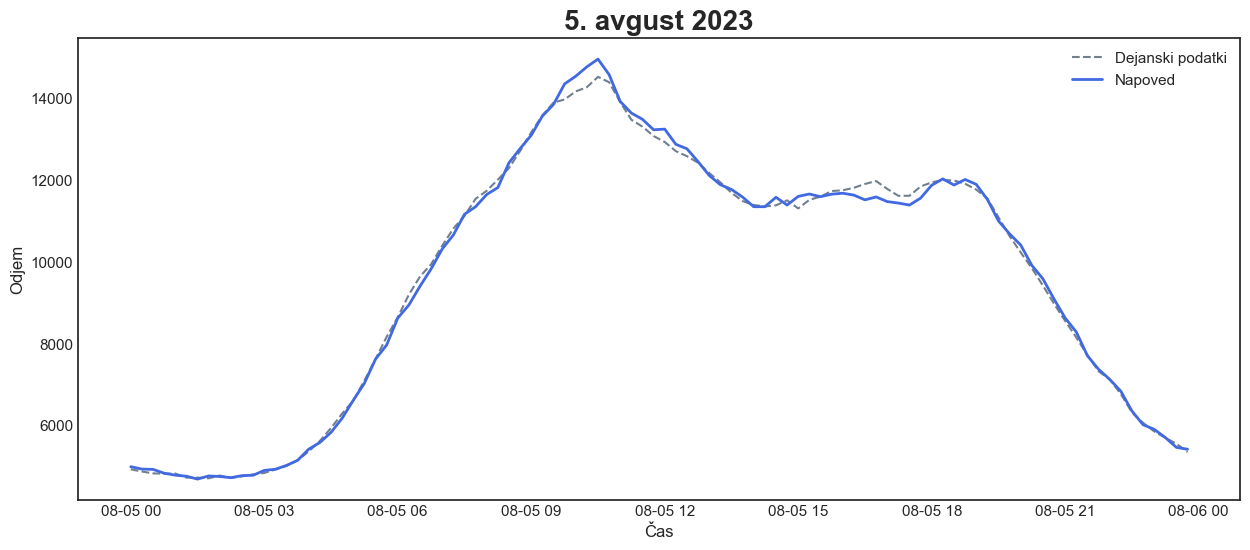
\includegraphics[width=\linewidth]{napoved_1.png}
        \end{minipage}
        \hfill
        \begin{minipage}[c]{0.48\linewidth}
            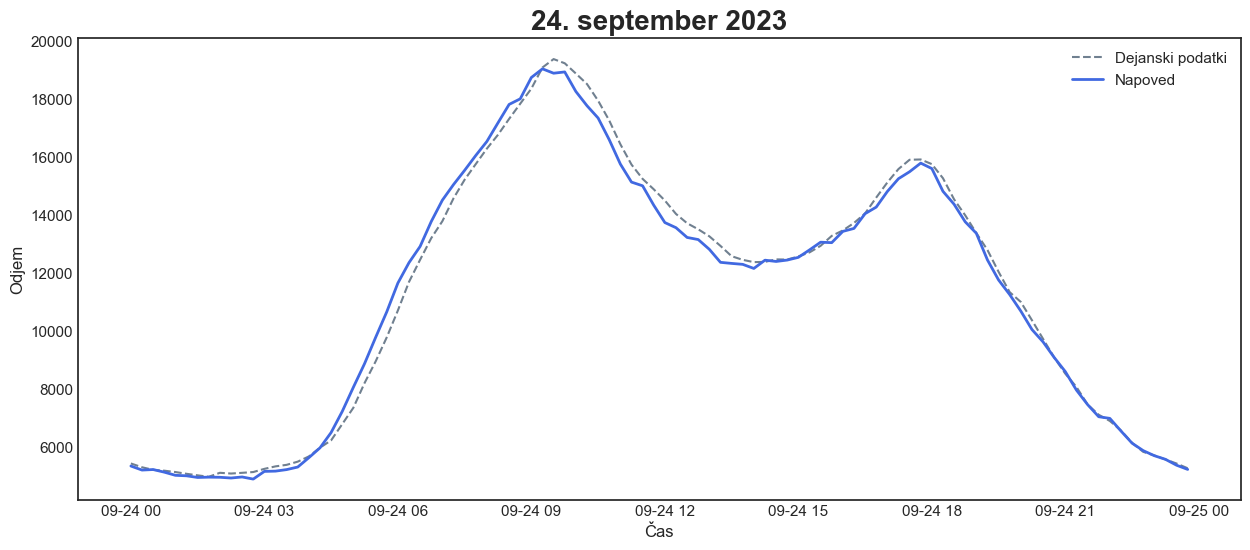
\includegraphics[width=\linewidth]{napoved_2.png}
        \end{minipage}
    \end{figure}
    \begin{figure}[!ht]
        \centering
        \begin{minipage}[c]{0.48\linewidth}
            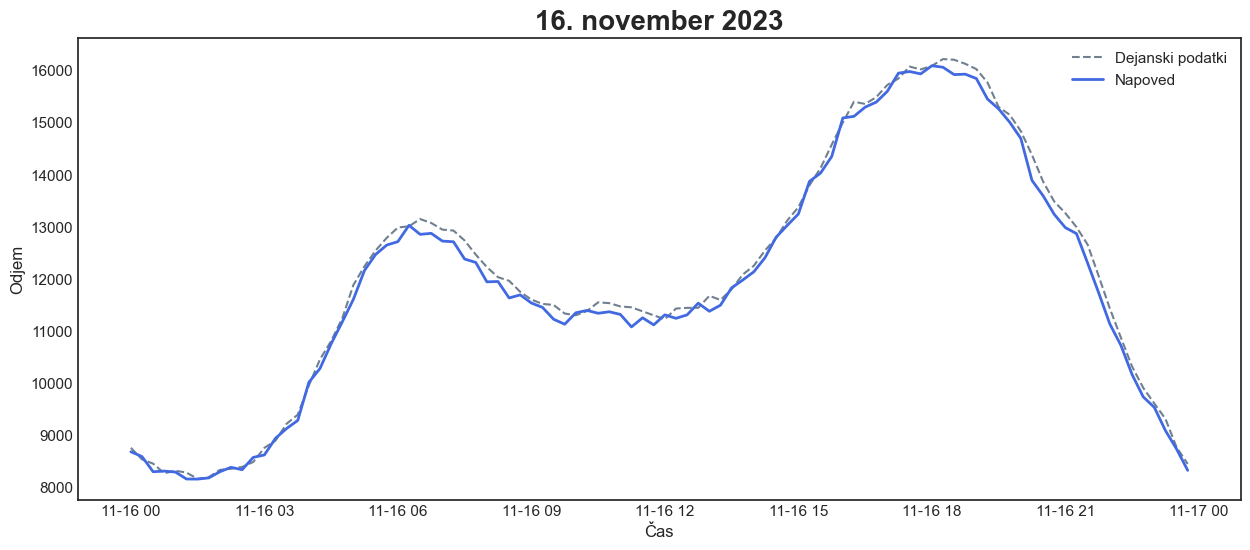
\includegraphics[width=\linewidth]{napoved_3.png}
        \end{minipage}
        \hfill
        \begin{minipage}[c]{0.48\linewidth}
            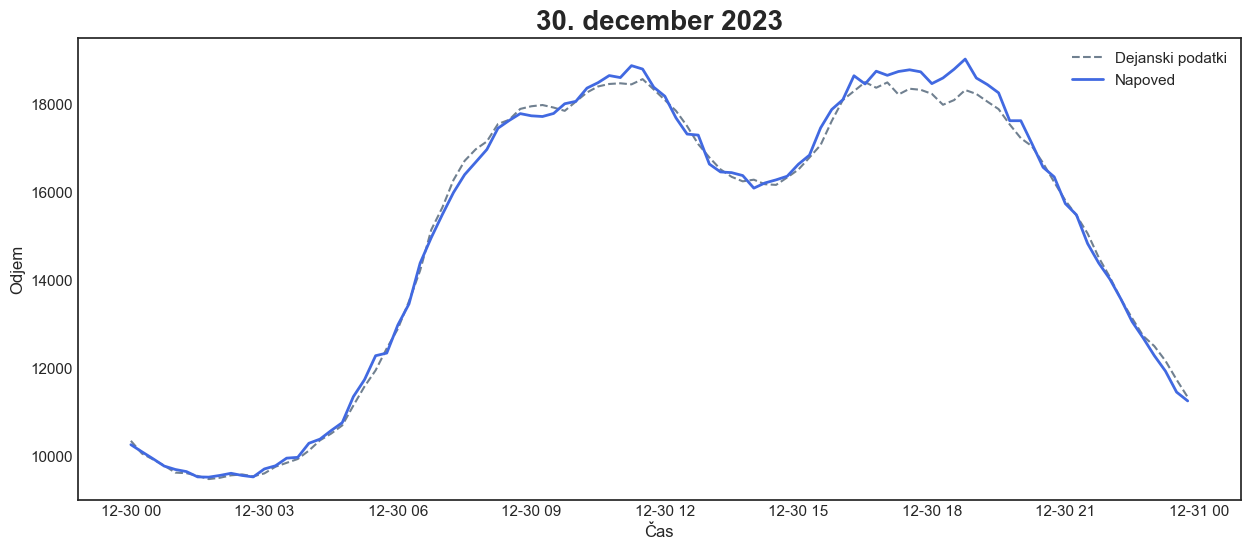
\includegraphics[width=\linewidth]{napoved_4.png}
        \end{minipage}
    \end{figure}

\end{frame}


% -------------------------------------------------------------------


\begin{frame}
    
    \frametitle{Napaki MAPE in RMSE} 

    Napaki RMSE (ang. \emph{Root-mean-square deviation}) in 
    MAPE (ang. \emph{Mean absolute percentage error}) izračunamo po formulah:
    
    $$
    RMSE = \sqrt{\frac{1}{96}\sum_{t=1}^{96}{(W_t-\hat{W_t})^2}} \quad \textrm{in} \quad
    MAPE = \frac{1}{96}\sum_{t=1}^{96}{\frac{W_t-\hat{W_t}}{W_t}} \,,
    $$
    
    \noindent kjer je $W_t$ dejanska vrednost odjema, $\hat{W_t}$ pa napovedana

\end{frame}


% -------------------------------------------------------------------


\begin{frame}
    
    \frametitle{Napaki MAPE in RMSE za izbrane datume} 

    \begin{table}[!ht]
        \footnotesize
        \centering
        \label{Tab:RMSE_MAPE}
        \begin{tabular}{l|c|c}
            Datum & RMSE & MAPE \\ \hline
            5. avgust 2023 & 156,600 & 1,104 \\ 
            24. september 2023 & 365,372 & 2,392 \\ 
            16. november 2023 & 176,901 & 1,199 \\ 
            30. december 2023 & 224,123 & 1,046 \\ 
            7. januar 2024 & 399,578 & 1,839 \\ 
            12. februar 2024 & 248,981 & 1,287 \\ \hline
            Povprečje & 261,926 & 1,478 \\ 
        \end{tabular}
    \end{table}

    \begin{itemize}
        \item Z vključitvijo še drugih primerov ugotovimo, da RMSE znaša okrog $260$, MAPE pa $1{,}5~\%$
        \item Vključitev eksogenih podatkov prispeva k bolj točni napovedi
    \end{itemize}

\end{frame}


% ===================================================================


\section{Zaključek}


% -------------------------------------------------------------------

\begin{frame}
    
    \frametitle{Zaključek} 

    \begin{itemize}
        \item Izbran model: SARIMAX(4,1,5)(0,1,0)[96]-GARCH(1,3)
        \item Dobre napovedi
        \item Z bolj zmogljivim računalnikom bi prišli do boljših rezultatov
        \item Funkcija \texttt{napoved\underline{\enskip}z\underline{\enskip}SARIMA\underline{\enskip}GARCH}
    \end{itemize}

\end{frame}


% -------------------------------------------------------------------

\begin{frame}
    
    \frametitle{Funkcija \texttt{napoved\underline{\enskip}z\underline{\enskip}SARIMA\underline{\enskip}GARCH}} 

    \begin{figure}[h!]
        \centering
        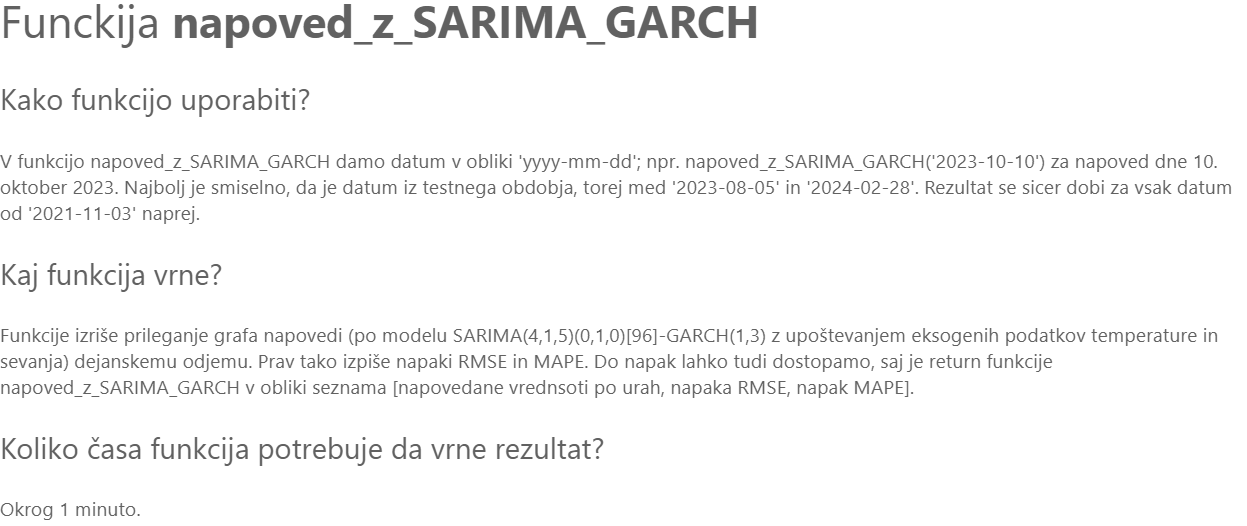
\includegraphics[width=0.9\textwidth]{opis_funkcije.png}
    \end{figure}

\end{frame}


% -------------------------------------------------------------------

\begin{frame}
    
    \frametitle{Primer uporabe \texttt{napoved\underline{\enskip}z\underline{\enskip}SARIMA\underline{\enskip}GARCH}} 

    \begin{figure}[h!]
        \centering
        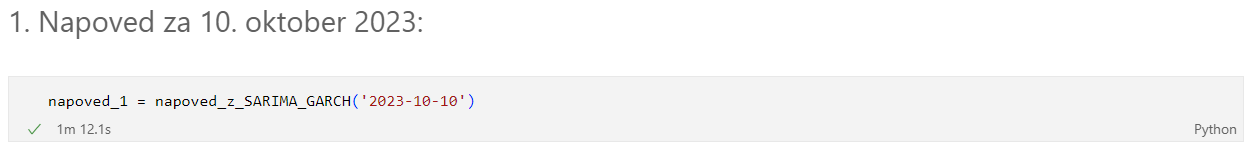
\includegraphics[width=0.9\textwidth]{koda.png}
    \end{figure}

    \begin{figure}[h!]
        \centering
        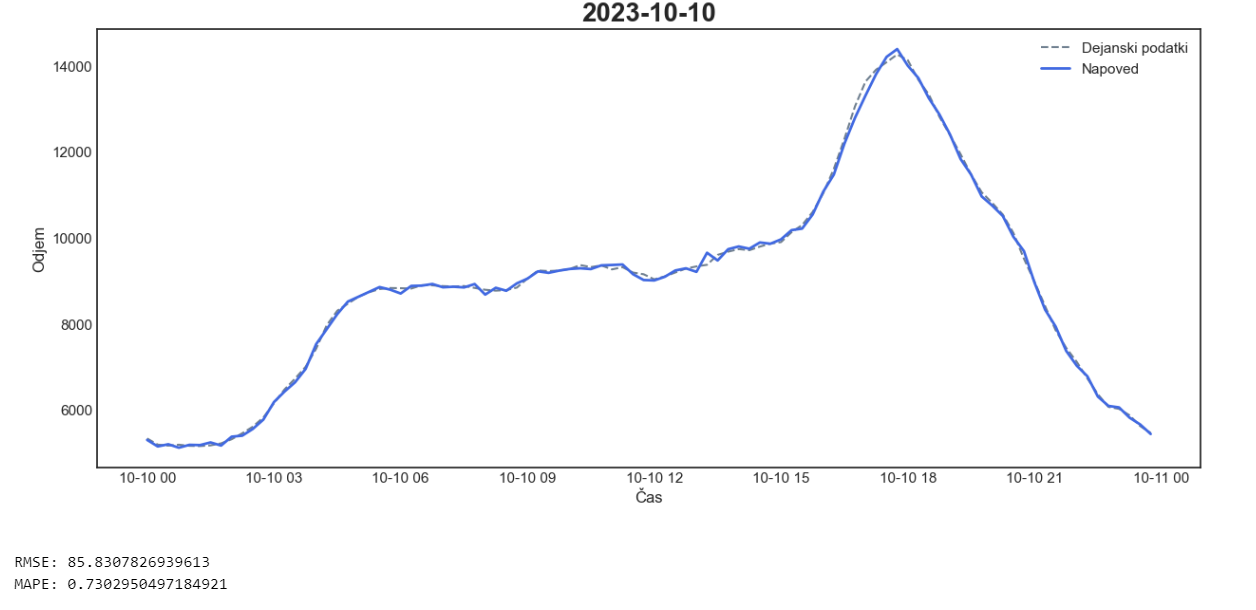
\includegraphics[width=0.9\textwidth]{izpis_funkcije.png}
    \end{figure}

\end{frame}


% -------------------------------------------------------------------





% -------------------------------------------------------------------



% ===================================================================

\end{document}
